\documentclass{article}

% if you need to pass options to natbib, use, e.g.:
%     \PassOptionsToPackage{numbers, compress}{natbib}
% before loading neurips_2024


% ready for submission
\usepackage{neurips_2024}


% to compile a preprint version, e.g., for submission to arXiv, add add the
% [preprint] option:
%     \usepackage[preprint]{neurips_2024}


% to compile a camera-ready version, add the [final] option, e.g.:
%     \usepackage[final]{neurips_2024}


% to avoid loading the natbib package, add option nonatbib:
%    \usepackage[nonatbib]{neurips_2024}

\usepackage{tikz}
\usepackage{courier} % for monospace font
\usepackage[utf8]{inputenc} % allow utf-8 input
\usepackage[T1]{fontenc}    % use 8-bit T1 fonts
\usepackage{hyperref}       % hyperlinks
\usepackage{url}            % simple URL typesetting
\usepackage{booktabs}       % professional-quality tables
\usepackage{amsfonts}       % blackboard math symbols
\usepackage{nicefrac}       % compact symbols for 1/2, etc.
\usepackage{microtype}      % microtypography
\usepackage{xcolor}         % colors


\title{Data Science Final Project: Laptop Price Analysis}


% The \author macro works with any number of authors. There are two commands
% used to separate the names and addresses of multiple authors: \And and \AND.
%
% Using \And between authors leaves it to LaTeX to determine where to break the
% lines. Using \AND forces a line break at that point. So, if LaTeX puts 3 of 4
% authors names on the first line, and the last on the second line, try using
% \AND instead of \And before the third author name.


\author{ \thanks{Use footnote for providing further information
    about author (webpage, alternative address)---\emph{not} for acknowledging
    funding agencies.} \\
  Anonymous Institution\\
  \texttt{anonymous@email.com} \\
}
  % Luca Hergan and Joe Loparco
  % \And
  % Coauthor \\
  % Affiliation \\
  % Address \\
  % \texttt{email} \\
  % \AND
  % Coauthor \\
  % Affiliation \\
  % Address \\
  % \texttt{email} \\
  % \And
  % Coauthor \\
  % Affiliation \\
  % Address \\
  % \texttt{email} \\
  % \And
  % Coauthor \\
  % Affiliation \\
  % Address \\
  % \texttt{email} \\
}


\begin{document}


\maketitle


\begin{abstract}
  This paper aims to investigate the relationship between laptop price and various laptop features. We employed the use of hot encoding to convert categorical data types to numerical. We go about this by splitting our data into train/test groups and then implementing two linear regression models with said groups. The models reveal the correlations between the price and other features in our data set. We found that the main hardware components, such as RAM, CPU, and GPU have the strongest impact on price. The accuracy of our model was limited by several things such as they way we hot encoded our categorical data, the inability 
  of linear regression to fit non-linear relationships, and the assumption of fair pricing of the laptops in our dataset across all time as components have progressed, and gotten cheaper. 
\end{abstract}

\section{Introduction}
For our final project we choose to perform a price analysis, and then price prediction of Laptops and using a linear regression model. We aimed to use this model to determine the effect that various features have on the overall price of a laptop. There are many reasons we felt compelled to do this such as the prevalence of laptops in everyday life and especially our own lives as computer scientists. This relevance is compounded by the fact that laptops are an incredibly expensive item that have a life span of multiple years, and thus it is pertinent that we and other consumers make good choices when it is time to buy.

\section{Pre-processing}

\subsection{Data Importing}


The data set we used for the project was of relatively high quality. This meant that it did not require much pre-processing. Since our data was encoded in Windows-1252, a legacy single-byte character encoding, we were forced to use a special command for import in pandas called 'encoding'.

\subsection{Data Engineering}

We then proceeded to data engineer our data. The first thing that we did was check for missing elements since they could have a significant impact on our model. We did not find any missing values, reinforcing our belief in the quality of the data set. We then hot-encoded the string features to obtain numerical values (GPU/CPU/Brand/Company/Laptop type/Laptop ID/Screen resolution/OS) and turned all strings which could be represented as integers or floats into integers or floats (Memory/Weight/Price). We also added a new column that measured the total storage capacity separately from the storage models because we thought that the difference between HDD and SSD would also have an impact on price (Figure 1).

\begin{figure}[!h]
    \centering
    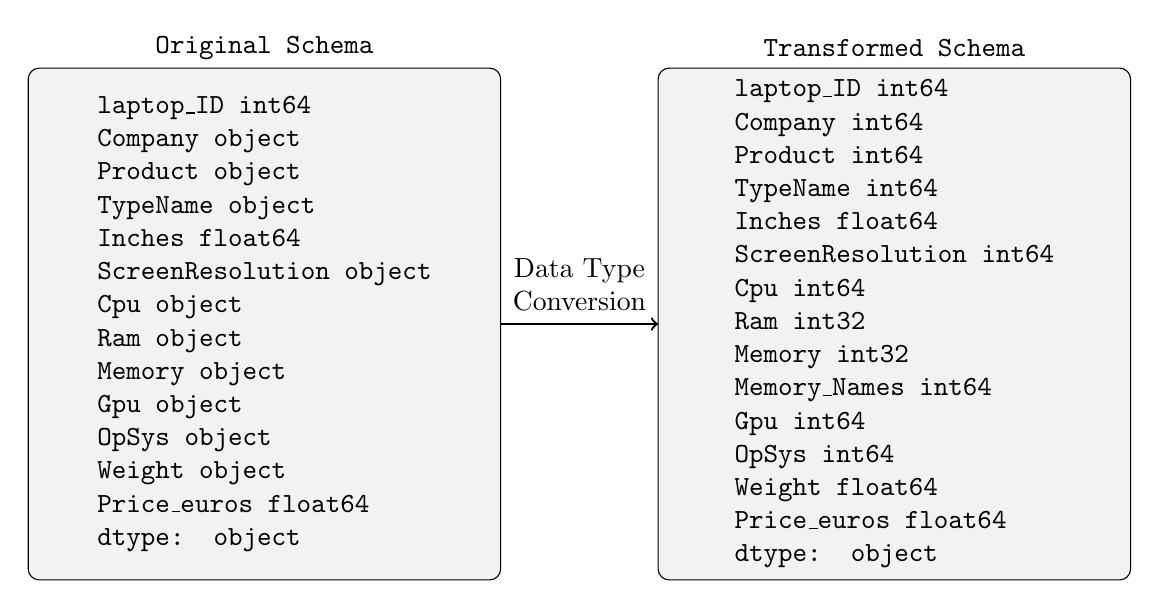
\begin{tikzpicture}
        % Left box
        \node[draw, rounded corners, fill=gray!10, minimum width=6cm, minimum height=6.5cm] at (0,0) {};
        \node[font=\bf\ttfamily] at (0,3.5) {Original Schema};
        
        % Right box
        \node[draw, rounded corners, fill=gray!10, minimum width=6cm, minimum height=6.5cm] at (8,0) {};
        \node[font=\bf\ttfamily] at (8,3.5) {Transformed Schema};
        
        % Left text
        \node[align=left,font=\ttfamily] at (0,0) {
            laptop\_ID      int64\\
            Company        object\\
            Product        object\\
            TypeName       object\\
            Inches         float64\\
            ScreenResolution object\\
            Cpu            object\\
            Ram            object\\
            Memory         object\\
            Gpu            object\\
            OpSys          object\\
            Weight         object\\
            Price\_euros    float64\\
            dtype: object
        };
        
        % Right text
        \node[align=left,font=\ttfamily] at (8,0) {
            laptop\_ID      int64\\
            Company        int64\\
            Product        int64\\
            TypeName       int64\\
            Inches         float64\\
            ScreenResolution int64\\
            Cpu            int64\\
            Ram            int32\\
            Memory         int32\\
            Memory\_Names   int64\\
            Gpu            int64\\
            OpSys          int64\\
            Weight         float64\\
            Price\_euros    float64\\
            dtype: object
        };
        
        % Arrow
        \draw[->,thick] (3,0) -- (5,0);
        \node[align=center] at (4,0.5) {Data Type\\Conversion};
    \end{tikzpicture}
    \caption{Data type transformation showing conversion from categorical objects to numeric encodings.}
    \label{fig:data-types}
\end{figure}

\section{Our Model: Linear Regression}
\label{gen_inst}

Using these engineered data, we then proceeded to build two different linear regression models. One used all data, including the hot encoded data, and the other only used numerical data. This was to check our suspicion that all data indeed contributed to the price, even non-numerical. (Figure 2)

\subsection{All Data}

The model incorporating all features, including hot-encoded categorical data, demonstrated stronger predictive performance compared to numerical data alone. With thirteen coefficients and an intercept of -181.705, this model achieved an $R^2$ score of 65.54\%, indicating that it explains approximately two-thirds of the variance in laptop prices. The model's mean absolute error of 302.80 euros suggests reasonable accuracy in price predictions, though the root mean squared error of 429.74 euros indicates some sensitivity to outliers and larger prediction errors on higher-priced laptops.

\begin{align*}
\begin{split}
\beta_1 &= 0.126 & \quad \beta_8 &= 77.940 \\
\beta_2 &= 8.405 & \quad \beta_9 &= 4.694 \\
\beta_3 &= 0.152 & \quad \beta_{10} &= -0.058 \\
\beta_4 &= 40.660 & \quad \beta_{11} &= 3.118 \\
\beta_5 &= -73.473 & \quad \beta_{12} &= 103.050 \\
\beta_6 &= 9.516 & \quad \beta_{13} &= 136.530 \\
\beta_7 &= 5.129 & \quad \text{intercept} &= -181.705
\end{split}
\end{align*}


\subsection{Numerical data}

The simplified model using only numerical features showed reduced but still meaningful predictive power. With three coefficients, which included RAM and total storage (named memory), had an intercept of 389.385. This model achieved an $R^2$ score of 56.62\%. The higher mean absolute error of 346.78 euros and root mean squared error of 482.12 euros compared to the full model suggests that categorical features like brand, GPU, and CPU specifications contain valuable information for price prediction that cannot be captured by numerical features alone.

\begin{align*}
\begin{split}
\beta_1 &= 107.235 \quad & \beta_3 &= -49.339 \\
\beta_2 &= -0.118 \quad & \text{intercept} &= 389.385
\end{split}
\end{align*}

\begin{figure}[!h]
    \centering
    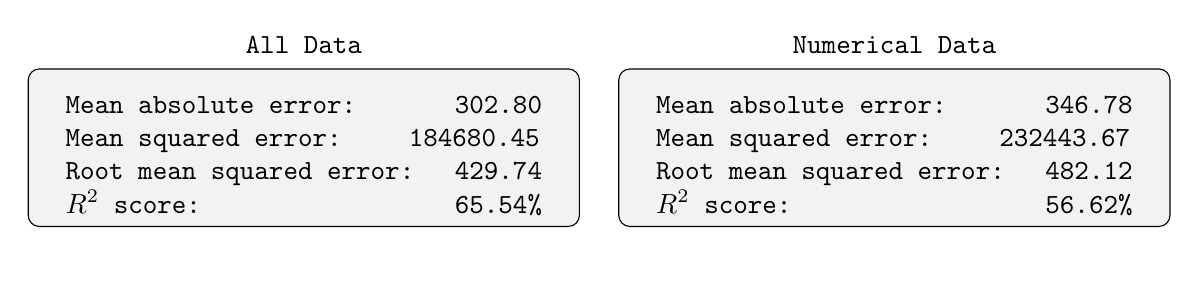
\begin{tikzpicture}
        % Left box
        \node[draw, rounded corners, fill=gray!10, minimum width=7cm, minimum height=2cm] at (0,0) {};
        \node[font=\bf\ttfamily] at (0,1.3) {All Data};
        
        % Right box
        \node[draw, rounded corners, fill=gray!10, minimum width=7cm, minimum height=2cm] at (7.5,0) {};
        \node[font=\bf\ttfamily] at (7.5,1.3) {Numerical Data};
        
        % Left text
        \node[align=left, font=\ttfamily] at (0,-0.3) {
            Mean absolute error:   \hspace*{.7cm}   302.80\\
            Mean squared error:     \hspace*{.3cm}   184680.45\\
            Root mean squared error:   \hfill     429.74\\
            $R^2$ score:   \hfill    65.54\%\\
        };
        
        % Right text
        \node[align=left, font=\ttfamily] at (7.5,-0.3) {
            Mean absolute error:   \hspace*{.7cm}   346.78\\
            Mean squared error:    \hspace*{.3cm}    232443.67\\
            Root mean squared error:  \hfill      482.12\\
            $R^2$ score:   \hfill    56.62\%\\
        };
        
    \end{tikzpicture}
    \caption{Results for both linear regression models}
    \label{fig:model-comparison}
\end{figure}

\section{Limitations}

\subsection{Model Limitations}

Linear regression is a relatively simple model and as a result has drawbacks. The first significant one that we encounter is its ability to measure non-linear relationships between various features. This can be seen in our residual graph as the prices for higher-end laptops are very rarely predicted near their true price. We believe this is due to how the pricing works in the market - a marginal gain on the highest end laptops can cause a significant increase in price. Since most of the model was trained on lower end laptops, it is more likely to minimize the loss for those occurrences, and so when left to estimate higher-end parts it does not have appropriate weighting.

\subsection{Data Limitations}

Our dataset and encoding present several notable limitations that could affect model accuracy. Our primary concern is our hot encoding approach for categorical variables. Here we made assumptions about the ordinal nature of certain features. For instance, our encoding of operating systems \{'Android': 0, 'Chrome OS': 1, 'Linux': 2, 'Mac OS X': 3, 'No OS': 4, 'Windows 10': 5, 'Windows 10 S': 6, 'Windows 7': 7, 'macOS': 8\}. This ordering implicitly suggests that Windows 7 is superior to Windows 10, and that having no operating system is preferable to having Android or Chrome OS. This is due to the increased prices by the first mentioned operating systems, and the cheaper nature of the second ones listed. These encoding decisions could introduce bias into our model by misrepresenting relationships between categorical variables. Additionally, our dataset might contain pricing anomalies or outliers from outdated listings or incorrectly priced items, potentially skewing our model's understanding of the non-linear relationship between component quality and price. This is particularly problematic given that we assumed all laptops in our dataset were priced fairly relative to their specifications. These data quality issues, combined with the inherent limitations of linear regression in handling non-linear relationships suggest that our model might be less reliable when predicting prices for high-end laptops where component quality and price relationships often become especially non-linear.

\section{Figures and Interpretations}
\label{others}
\begin{figure}[!h]
    \centering
    \begin{minipage}{0.45\textwidth}
        \centering
        \includegraphics[width=\linewidth]{Price Distribution.png}
        \caption{Price Distribution}
        \label{fig:price-dist}
    \end{minipage}%
    \hfill
    \begin{minipage}{0.45\textwidth}
        \centering
        \includegraphics[width=\linewidth]{Weight Distribution.png}
        \caption{Weight Distribution}
        \label{fig:weight-dist}
    \end{minipage}
\end{figure}

\begin{figure}
    \centering
    \includegraphics[width=1\linewidth]{Confusion Matrix.png}
    \caption{Confusion Matrix}
    \label{fig:enter-label}
\end{figure}

\begin{figure}
    \centering
    \includegraphics[width=1.15\linewidth]{Residual Plot.png}
    \caption{Plot of Residuals}
    \label{fig:enter-label}
\end{figure}


\subsection{Price Distribution}
The price distribution appears to be uni-modally distributed as there is only one peak in our data. Our data also skews heavily to the right due to the presence of a lower limit as nothing can have a price lower than 0\$. (Figure 3)

\subsection{Weight Distribution}
The weight distribution is tri-modally distributed as there appear to be several clusters in our distribution chart where local maxima exist displayed by our curve. We are unsure as to why this clustering manifested the way it did in our distribution, but one possible reason could be because there are different types of laptops (i.e. Notebook, Gaming, Etc.) and these laptops are likely to have  mean weights similar to other of their type as their requirements align in terms of features and consequentially categorization. One example of this would be gaming laptops which would require more robust hardware and therefore are more likely to define the third local maximum in weight along with workstations. (Figure 4)

\subsection{Confusion Matrix}
Above you can see the confusion matrix which shows the linear relationship between the various features of our data set. The price column is the column that pertains to our analysis. As you can see in the figure above the feature that had the strongest correlation with price was RAM (measured by capacity in GB not speed in mHz), followed by CPU model (categorically) and then GPU (categorically). This is what we expected prior to our analysis as these are the most expensive individual components in the laptop, and thus it makes sense that and increase in the quality of these components would lead to a significant increase in price. RAM had a correlation coefficient of .743. This shows that RAM capacity directly and linearly contributes a significant amount to the final price of a laptop. (Figure 5)

\subsection{Residual Plots}
The distribution of our residuals appears to be approximately normal and uni-modal with a slight skew right. The chart of residuals vs predicted values appears to be shaped how we would expect, with greater residuals and therefore inaccuracy on higher priced laptops. We think this is due to the marginal performance gain relative to increase in price for higher end products. (Figure 6)


\section{Conclusion}
In this project we conducted a statistical analysis on the price of laptops, and which factors contribute most to said price. Our motivation for this project was the prevalence of laptops in our personal and educational lives. We aimed to predict the price of laptops by training and testing two separate linear regression models. We did this by splitting our pre-processed data into train and test categories, and assessing our performance on the test data after fitting our models. Our results showed us that the main hardware components, RAM, CPU, and GPU in decreasing order, have the strongest correlation to the price of a laptop. Despite our models being relatively accurate, we ran into several limitations throughout the course of this project. These limitations range from the inability of our model to fit onto non-linear relationships. Adding to this, our model was also limited by our implementation of hot-encoding and the assumption of fair pricing close to market suggested retail price. In conclusion the price of a laptop is affected by many features but is most greatly affected by the choice of hardware components. 


\end{document}